\section{Simulation Studies}

The simulation study was broken up in two separate experiments: (1) the first was used to define a baseline comparison 
of the methods on multivariate normal data in both high and low dimensional conditions; (2) the second was used to 
assess the performance of the methods in the presence of a latent structure, in order to reflect the fundamental
structure of social survey data.

\subsection{Simulation Study Procedure}
	
	To assess the statistical validity of the different imputation methods we have repeated the following steps
	1000 times for each experiment:

	\begin{enumerate}
		\item Data generation: A data matrix $\bm{Z}_{n \times p}$ was generated according to an experiment 
			specific data generating model (e.g. multivariate normal model, confirmatory factor analysis),
			the characteristics of which depend on experimental conditions described below.
		\item Missing data imposition: Missing values were imposed on a given number of target variables
			in $\bm{Z}_{n \times p}$, according to some response model.
		\item Imputations: Each method described in section 2 to deal with missing values was used for 
			imputation.
		\item Analysis: Different analysis models were fitted to the differently treated data.
			Parameters estimates were pooled across the differently imputed datasets, for the MI methods,
			and stored along with the estimates obtained with single imputation methods and complete case 
			analysis.
	\end{enumerate}

	The code to Run the simulation was written in the R statistical programming language (version 4.0.3). 
	All experiments were run using a 2.6 GHz Intel Xeon(R) Gold 6126 processor, 523780 MB of Memory. The
	operating system was Windows Server 2012 R2.

	Computations were run in parallel across 30 cores. 
	Parallel computing was implemented using the R package \emph{parallel} and to ensure replicability 
	of the findings seeds were set using the method by \cite{lecuyer:2002} implemented in the R package 
	\emph{rlecuyer}.
	Code to run the studies can be found at \url{https://github.com/EdoardoCostantini/imputeHD-comp}.

	In the following, each step of the simulation procedure is described in details for both experiments.

%\subsection{Methods: two simulation studies}

\subsubsection{Step 1: Data generations}

	\paragraph{Experiment 1} 
	The $\bm{Z}_{n \times p}$ data matrix in step 1 was generated by drawing from a multivariate normal 
	distribution centered around 0 with a covariance matrix $\bm{\Sigma}_0$, with diagonal elements 
	(variances) equal to 1. 
	The off-diagonal elements of $\bm{\Sigma}_0$ were used to define three blocks of variables: 
	the first five variables were highly correlated among themselves ($\rho = .6$); 
	variables 6 to 10 were slightly correlated with variables in block 1 and among themselves ($\rho = .3$), 
	and all the remaining $p-10$ variables were uncorrelated.
	Items were rescaled to have mean of 5.

	\paragraph{Experiment 2}
	The observed data $\bm{Z}_{n \times p}$ was created based on a Confirmatory Factor Analysis model.
	Each of $l$ latent variables was assumed to be measured by 5 items, for a total of $p = 5 \times l$ 
	columns in $\bm{Z}$.
	Values on the observed items for the $i$-th observation were obtained with the following measurement 
	model:

	\begin{equation}
		\bm{z}_i = \bm{\Lambda} \bm{\xi}_{i.} + \bm{\delta}_{i.}
	\end{equation}

	where $\bm{z}_i$ is a vector of $5 \times l$ observed items scores, for observations $i = 1, ..., n$;
	$\bm{\Lambda}$ is the matrix of factor loadings; $\bm{\xi}_{i.}$ is a vector of scores on the
	latent variables for observation $i$; and $\bm{\delta}_{i.}$ is a vector of uncorrelated multivariate 
	normal measurement errors.
	For notation and model specification the interested reader may refer to \cite{bollen:1989}.
	All items are centered around a mean value of 5.

	The latent scores in $\bm{\xi}_{i.}$ are sampled from a multivariate normal distribution centered around 
	0, and with a covariance matrix $\bm{\Psi}_0$, with diagonal elements equal to 1 and off-diagonal elements 
	equal to correlation between latent factors. 
	In particular, the first 4 latent variables are highly correlated ($\rho = .6$), the second block of 4 
	latent variables are somewhat correlated ($\rho = .3$), while the remaining $l-8$ latent variables are 
	uncorrelated.

	The matrix $\bm{\Lambda}$ defines a simple latent structure where each item loads on only 1 factor (5 items 
	for each latent variable).
	Both the item and latent factor variances are set to 1, $var(x_i) = 1$ and $\Psi_{ii} = 1$, so that 
	the measurement error is defined as $var(\delta) = 1 - \lambda^{2} 1$. 
	This specification allows factor loadings $\lambda_{ij}$, with $i = 1, ..., n$ and $j = 1, ..., l$, to be
	defined as standardized values that range between 0 and 1.
	If all values in $\bm{\Lambda}$ are 0s, there is no latent structure and items are simply drawn from  
	multivariate distribution centered around the item means with covariance matrix $\bm{\Psi}_0$.
	If all values in $\bm{\Lambda}$ are 1s, there is a \emph{prefect} latent structure, meaning that items
	exactly measure the latent constructs.
	The exact values for the latent factors are drawn for each repetition from a uniform distribution between
	a lower and upper bound, $b_l$ and $b_u$, that are condition-specific (see below).

	\paragraph{Conditions}
	
	The data generating mechanisms described above were specified according to different conditions which are
	described below.
	Table \ref{table:condSum} summarizes these conditions.

	\paragraph{Experiment 1}
	In experiment 1, the sample size $n$ was set to 200 in all conditions.
	Two experimental factors were considered: $p$, the number of columns in the dataset which are all fed to the 
	imputation algorithms, taking value 50 or 500; 
	and $pm$, the target proportion of \emph{per} variable missing cases, taking value 0.1 or 0.3

	\paragraph{Experiment 2}
	The dimensionality of the data was controlled based on the number of latent variables $l$.
	Two values were used for this factor: 10 and 100. 
	In all conditions, 5 items were generated as measures for each latent variable, making conditions with $l = 10$ 
	low dimensional conditions, with 50 total predictors and a constant sample size of 200 observations, and 
	conditions with $l = 100$ high dimensional ones, with data matrices of dimensionality $200 \times 500$.
	The proportion of missing values was defined again as a fixed experimental factor with two levels: 0.1 or 0.3.

	In experiment 2, we also defined the factor loadings $\lambda_{ij}$ as a 2-level random experimental factor.
	The data generation step used factor loadings drawn from a uniform distribution defined by a lower and upper bound 
	$(b_l, b_u)$, taking values either high $(0.9, 0.97)$ or low $(0.5, 0.6)$.

\begin{table}[h]
   \begin{center}
        \begin{tabular}{ c c c c c c }
		% Column names
		\textbf{condition} & \textbf{n} & \textbf{p} & \textbf{l} & \textbf{pm} & \textbf{$\lambda$ range} \\ 
		\hline

		% Group name
		\rowcolor{Gray}
 		\multicolumn{6}{c}{Experiment 1} \\
		\hline

		% Row 1
		1 & 200 & 50  & - & .1 & - \\
		2 & 200 & 500 & - & .1 & - \\
		3 & 200 & 50  & - & .3 & - \\
		4 & 200 & 500 & - & .3 & - \\

		\hline

		& & & & & \\ 

		% Group Name
		\rowcolor{Gray}
 		\multicolumn{6}{c}{Experiment 2} \\
		\hline

		1 & 200 & 50 &  10 &  0.1 & [.9, .97] \\
		2 & 200 & 500 & 100 & 0.1 & [.9, .97] \\
		3 & 200 & 50 &  10 &  0.3 & [.9, .97] \\
		4 & 200 & 500 & 100 & 0.3 & [.9, .97] \\
		5 & 200 & 50 &  10 &  0.1 & [.5, .6]  \\
		6 & 200 & 500 & 100 & 0.1 & [.5, .6]  \\
		7 & 200 & 50 &  10 &  0.3 & [.5, .6]  \\
		8 & 200 & 500 & 100 & 0.3 & [.5, .6]  \\

		\hline
        \end{tabular}
    \end{center}
\caption{Summary of conditions for experiment 1 and 2} \label{table:condSum}
\end{table}

\FloatBarrier % stops table:condSum leaving its own section

\subsubsection{Step 2: Missing data imposition} \label{sub_missing}

	The non-response mechanism was modelled as a logistic regression:

	\begin{equation}
		logit[p(z_{i,j} = miss | Z)] = \theta_0 + \tilde{Z}_{i}\bm{\theta}
	\end{equation}
	
	where $z_{i,j}$ is the $i$-th subject's response on the $j$-th variable, $\theta_0$ is the intercept parameter,
	$\tilde{Z}_{i}$ is a vector of responses for the $i$-th individual to the set of predictors involved in the
	missing data mechanism, and $\bm{\theta}$ is the vector of slope parameters.
	The probability of an individual non response was computed as the inverse of the logit function as

	\begin{equation} \label{eqn:rm}
		p_{miss} = p(z_{i,t} = miss | X) = \frac{ exp(\theta_0 + \tilde{Z}\bm{\theta}) }
								{ 1 + exp(\theta_0 + \tilde{Z}\bm{\theta}) }
	\end{equation}

	Finally, an $n$ dimensional response vector was sampled from a binomial distribution $b(n, p_{miss})$.
	The value of $\theta_0$ was chosen with an optimization algorithm that minimized the difference between a 
	target proportion of missing values and its actual value.

	\paragraph{Experiment 1}
	Six variables were chosen as target of missing data imposition: three variables in the block of
	highly correlated variables and three in the block of lowly correlated variables ($z_j$ with $j = 1,2,3,6,7,8$).
	Item non-response was imposed by sampling from a binomial distribution with non-response probabilities computed 
	with equation (\ref{eqn:rm}). 
	$\tilde{Z}$ was specified to include two fully observed variables from the highly correlated set, and two 
	from the lowly correlated set ($z_r$ with $r = 4,5,9,10$).

	The choice of predictors in $\tilde{Z}$ is important to allow imputations under MAR: 
	the probability of observing a response for a target variable did not depend on the variable itself, 
	to avoid imputation under Missing Not At Random; and, as all features in the data are included in the MI 
	procedures, the predictors in $\tilde{Z}$ are always allowed to be part of the imputation models.

	\paragraph{Experiment 2}
	Item non-response was imposed on the 10 items measuring two highly correlated latent variables ($l = 1, 2$) 
	using the other two highly correlated latent variables ($l = 3, 4$) as predictors in response model (\ref{eqn:rm}). 

\subsubsection{Step 3: Imputation}
	
	Missing values were treated with all the methods described in section 2.
	Here, we describe some key details in the algorithms specifications.

	\paragraph{Convergence}

	For both experiments, convergence of the imputations was assessed in a preprocessing step.
	Before running the actual simulation studies, 10 datasets were generated according to each experimental set up.
	Missing values in each dataset were imputed by running 5 parallel imputation chains for each Multiple Imputation 
	method.
	Convergence was checked by plotting the mean of the imputed values for each variable in each stream, against the 
	iteration number.

	This procedure was performed only for the condition with larger proportion of missing values and larger number of 
	predictors.
	Being this the most challenging condition for the imputation task, the decisions made for this condition were
	applied to the simpler ones.

	In each parallel run, all the MI algorithms run for 250 iterations.
	This number should be more then enough to check convergence of the MICE algorithms as in practice MICE requires 
	a much lower number of iterations than more traditional MCMC algorithms \citep[p. 126]{vanBuuren:2018}.
	After approximately 40 iterations, the patterns shown in these trace-plots were free of trend, and the variance 
	within chains was approximately the same as the variance between chains.
	Hence, to run the actual simulation experiments, the algorithms were considered to converge after 50 iterations, 
	after which 10 imputed data sets were store and used for the subsequent standard complete-data analysis and 
	pooling.

	It was expected that blasso would require more iterations to converge than the other methods: the MCMC algorithm
	has to sample the penalty parameter $\tau$ and the sparsity parameter $\rho$ on top of all the other parameters 
	of the imputation models and the missing values replacements.
	Hence, to check convergence, each of the 5 parallel runs of the Blasso imputation algorithm run for a total 
	of 2000 iterations.
	For most variables and data repetitions, 500 iterations were more than enough to reach convergence of the 
	imputations.
	However, some exceptions required more than 1250 iterations to be free of trends.
	Hence, in the single chain run used to obtain the simulation results, the 10 datasets used for complete-data 
	analysis were kept after 1950 iterations of the blasso algorithm.
	Although this might seem a large number, blasso is a quite fast algorithm that allows this large number of iterations,
	at least in our set up.

	\paragraph{Tuning penalty parameters}

	The ridge penalty used in the bridge algorithm is fixed across iterations and its value needs to be
	decided beforehand by the imputer.
	The value used in the simulation was decided by means of cross-validation in a pre-processing phase.
	A grid of plausible values for the ridge penalty was defined by eight values equally spaced in the range from 
	$10^{-1}$ to $10^{-8}$. 
	For each of 100 data repetitions, bridge imputation was performed with each of the different penalty parameters
	and used to obtain 10 differently imputed datasets.
	For each data replication, the Fraction of Missing Information (fmi) \citep{savaleiRhemtulla:2012} associated with each 
	parameter in the analysis models of interest (see next section for details) was computed and then averaged across 
	repetitions.
	The mean of these average parameter fmis was used as a composite measure of fmi associated with each ridge penalty
	value.
	Finally, the penalty value with the smallest composite fmi was selected.
		
	Both IURR and DURR could have been specified with a variety of penalty parameters, from ridge to 
	elastic net penalties.
	In this study we specified the regularization as a lasso penalty, instead of a more elaborate elastic net, as
	the performance of the two were quite similar in \cite{zhaoLong:2016} and \cite{dengEtAl:2016} and the 
	cross-validation is less computationally intensive for the former.
	A 10-fold cross-validation procedure was used at every iteration of DURR and IURR to choose the penalty parameter.

	\paragraph{Blasso hyperparameters}

	For blasso, in order to maintain consistency with previous research, the hyperparameters in \ref{eqn:sigprior},
	\ref{eqn:tauprior}, and \ref{eqn:rhoprior} were specified as in \cite{zhaoLong:2016}: $(a,b)=(0.1, 0.1)$, 
	$(r,s)=(0.01, 0.01)$, and $(g,h)=(1,1)$.

	\paragraph{MI-PCA Number of components}

	In the MI-PCA algorithm, enough components were extracted to explain 50\% of the total variance in the data.

	\paragraph{missForest iterations and number of trees}

	To impute data with the single imputation random forest approach we provided the data
	with missing values to the function \emph{missForest} in the homonymous R package.
	This function implements algorithm 1 in \cite{stekhovenBuhlmann:2011}.
	The stopping criteria for the missForest algorithm was usually met under 10 iterations, but to make a
	conservative choice we fixed the maximum number of iterations to 20.
	\cite{stekhovenBuhlmann:2011} showed that increasing the number of trees grown in each forest has 
	stagnating effects on the imputation error while increasing linearly the computation time.
	In their paper, the authors recommend growing 100 trees per forest, which offers a good compromise 
	between imputation precision and computation time.
	Therefore, that is the value we used in this paper.

\subsubsection{Step 4: Analysis}
	
	\paragraph{Experiment 1}
	The substantive model of interest in experiment 1 was a saturated model that estimates means,
	variances, and covariances of the six variables with missing values.

	\paragraph{Experiment 2}
	The same saturated model was fitted to estimate the means, variances, and covariances of the 
	\emph{observed} items.
	Furthermore, the true Confirmatory Factor Analysis was also chosen to see how the factor loadings 
	are recovered after imputation.

\subsection{Comparison Criteria} \label{criteria}

	After running the simulation procedure $R=1000$ times, the $R$ Gold Standard estimates, obtained by saving the model 
	parameter estimates computed on the fully observed data, were averaged to define the true parameters values 
	in each condition.
	The $R$ estimates obtained by estimating the parameters of interest, after treating the missing values with all other 
	methods, were used to compute the methods performance measures.
	In what follows, we describe the outcome measures considered.

	\paragraph{Bias}

	First, we used the Percent Relative Bias ($PRB$) to quantify the bias introduced by 
	the imputation procedures:

	\begin{equation} \label{eqn:prb}
		PRB = \frac{\bar{\hat{\theta}} - \theta}{\theta} \times 100
	\end{equation}
	
	where $\theta$ is the \emph{true} value of the focal parameter (e.g. mean of item 1, variance of item 2)
	computed as 
	$\sum_{r=1}^{R} \hat{\theta}_{r}^{GS}/R$
	, with
	$\hat{\theta}_{r}^{GS}$ 
	being the Gold Standard parameter estimate for the \emph{r}-th repetition. 
	$\bar{\hat{\theta}}$ represents the focal parameter estimate under a given imputation method, averaged over 
	the MCMC replications, computed as
	$\sum_{r=1}^{R} \hat{\theta}_{r}/R$,
	with
	$\hat{\theta}_{r}$ being the estimate obtained after using a given imputation approach in the 
	\emph{r}-th repetition.
	PRBs larger than 10\% in absolute value were considered as extreme.

	\paragraph{Confidence Intervals Coverage}
	To assess the integrity of hypothesis testing, the Confidence Interval Coverage of the reference value
	was considered as

	\begin{equation} \label{eqn:cic}
		CIC =  \frac{ \sum_{r=1}^{R} I(\hat{\theta} \in \widehat{CI}_r ) }{R}
	\end{equation}

	where $\theta$ and $\widehat{CI}_r$ are, respectively, the parameter estimate and confidence interval of
	the focal parameter in a given repetition, 
	and $I(.)$ is the indicator function that returns 1 if the argument is true and 0 otherwise.

	CICs below .9 are usually considered problematic for 95\% confidence intervals \cite[p. 52]{vanBuuren:2018} 
	as they imply inflated Type I error rates.
	A high coverage (e.g., .99) may indicate confidence intervals that are too wide, implying that
	the imputation method leads to more conservative inferential conclusions, and in this sense it is less worrisome 
	than lower-than-nominal coverage.
	Therefore, Confidence Intervals were considered to show severe under-coverage (over-coverage) if they are 
	below 0.9 (above 0.99).

	In the present work, we also followed \cite{burtonEtAl:2006} and considered as problematic CI coverage rates
	outside of two Standard Errors (SE) of the nominal coverage probability (p).
	The standard error of nominal coverage is defined as $SE(p) = \sqrt{p (1-p)/R}$, with $p = .95$.
	Therefore, for $R = 1000$, CI coverages outside of the range (0.94, .96) were considered showing mild
	signs of deviation from nominal coverage.

\subsection{Results}

\subsubsection{Experiment 1}

	Figure \ref{fig:exp1bias} and \ref{fig:exp1cir} report the Percentage Relative 
	Bias and Confidence Interval Coverage, respectively, for each parameter estimate in the saturated model described 
	above.
	In the figures, single horizontal lines, representing the PRB (or CIC) of a parameter estimate for a single variable, 
	combine to form larger horizontal bars giving an aggregate account of how each method performed across
	multiple variables with missing values.

	\paragraph{Means} 
	Focusing first on the item means (top rows), all methods achieved a bias that is smaller than the 10\% threshold 
	for all item means, in all conditions.
	Looking at relative performances, in all conditions, MI-OP provided negligible bias, and IURR and MI-PCA resulted 
	in the smallest estimation bias among the other methods.

	In the conditions with high proportion of missing values (condition 3 and 4), all methods showed some signs of 
	95\% CI under-coverage of the true values, with CIC outside of the interval $(.94, .96)$.
	The only exceptions to the trend were MI-OP, MI-PCA, and Bridge which showed little deviation from nominal coverage.

	\paragraph{Variances} 
	Moving to the item variances (central rows), IURR, Blasso, and the tree based methods gave the lowest
	biases across all conditions, even in the most challenging one (condition 4).
	These low biases were mostly paired with low deviations from nominal coverage, except for condition 4 where 
	IURR and the tree based methods showed clear signs of under-coverage of the true item variances ($CIC << .9$).
	Apart from MI-OP, Blasso was the method with best coverage in this final condition.
	
	Directly using regularized regression within the imputation models (DURR) showed poor performances with regards 
	to variances: in all conditions but the first, it led to large (negative) bias, with a PRB as large as 10\% in 
	the last condition, accompanied by clear signs of CI under-coverage.
	Bridge was the only MI method showing larger bias than DURR, in all the high-dimensional conditions (2 and 4):
	imputing the data with Bridge led to all item variance estimates showing a bias larger than 20\% the size of the
	true value.

	MI-PCA also showed poor performances with a noticeable positive bias in all conditions that became extreme in
	condition 4, where the PRBs exceeded 20\%.
	This poor performance was reflected in extreme confidence interval under-coverage of the true item variances in
	the final experimental condition.

	Single data imputation with missForest and complete case analysis led to substantial negative bias and 
	CI under-coverage for all item variances, even in condition 1.

	\paragraph{Covariances}
	Finally, the third row in figure \ref{fig:exp1bias} shows the estimation bias for the 15 covariances between 
	the 6 items with missing values.
	As covariances depend on two variables, recovering the correct estimates after imputation is inherently 
	more difficult than with means and variances.
	This explains the generally worse performances reported in the figure.

	Indirect Use of Regularized Regression (IURR) performed noticeably better than most other methods, 
	with negligible negative bias and acceptable coverage for all covariances in conditions 1, 2 and 3, 
	but it struggled with a large negative bias and extreme under-coverage for the majority of the 15 
	covariances in condition 4.
	
	MI-PCA showed negligible negative biases of the covariance estimates in all conditions, performing as 
	well as MI-OP in all but the last condition, where it still maintained acceptably low values of PRB 
	($|PRB| < 10\%$).
	Furthermore, MI-PCA showed virtually no deviation from nominal coverage, with a CIC pattern similar to 
	that of MI-OP, in all but the last condition, where it manifested only mild \emph{over}-coverage of the 
	items covariances.

	All other methods, including DURR, showed absolute PRBs larger than the 10\% threshold in all but the 
	first condition, with mild to extreme signs of under-coverage.
	Bridge displayed acceptably low biases and coverage in the low dimensional conditions, and 
	extremely large biases and low CI coverage in all the high dimensional conditions.
	Single data approaches, like missForest and CC, showed extreme bias and under-coverage of covariances between 
	items with missing values, even in condition 1.
	

%\begin{landscape}
%\begin{rotatepage}
\begin{figure}[p]
	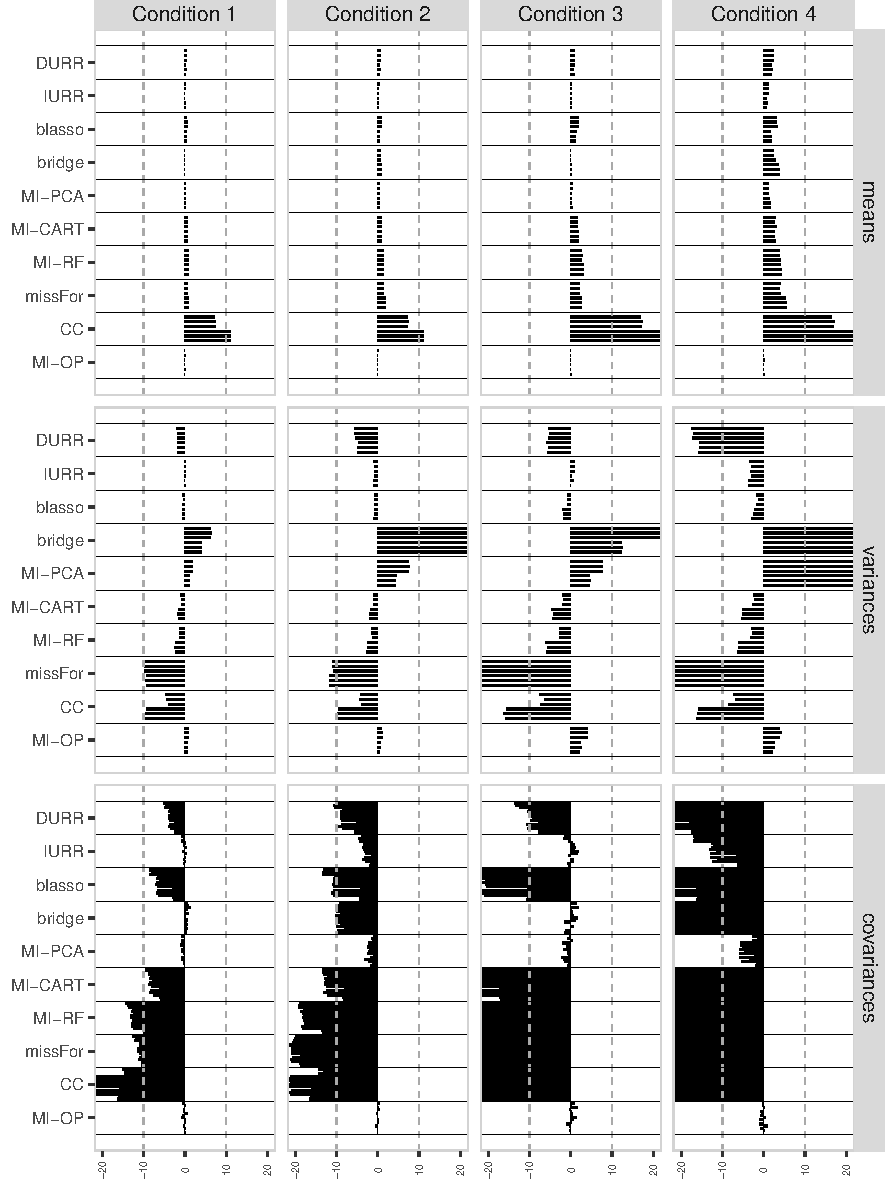
\includegraphics{../../output/graphs/exp1_bias.pdf}
\caption{
	Percent Relative Bias (PRB) for item means, variances, and covariances.
	For every method, single horizontal lines, representing the PRB of a parameter estimate on 
	a single variable (or pair of variables), combine to form larger horizontal bars giving an 
	aggregate account of how each method performed across multiple variables with missing values.
	}
\label{fig:exp1bias}
\end{figure}

\begin{figure}[p]
	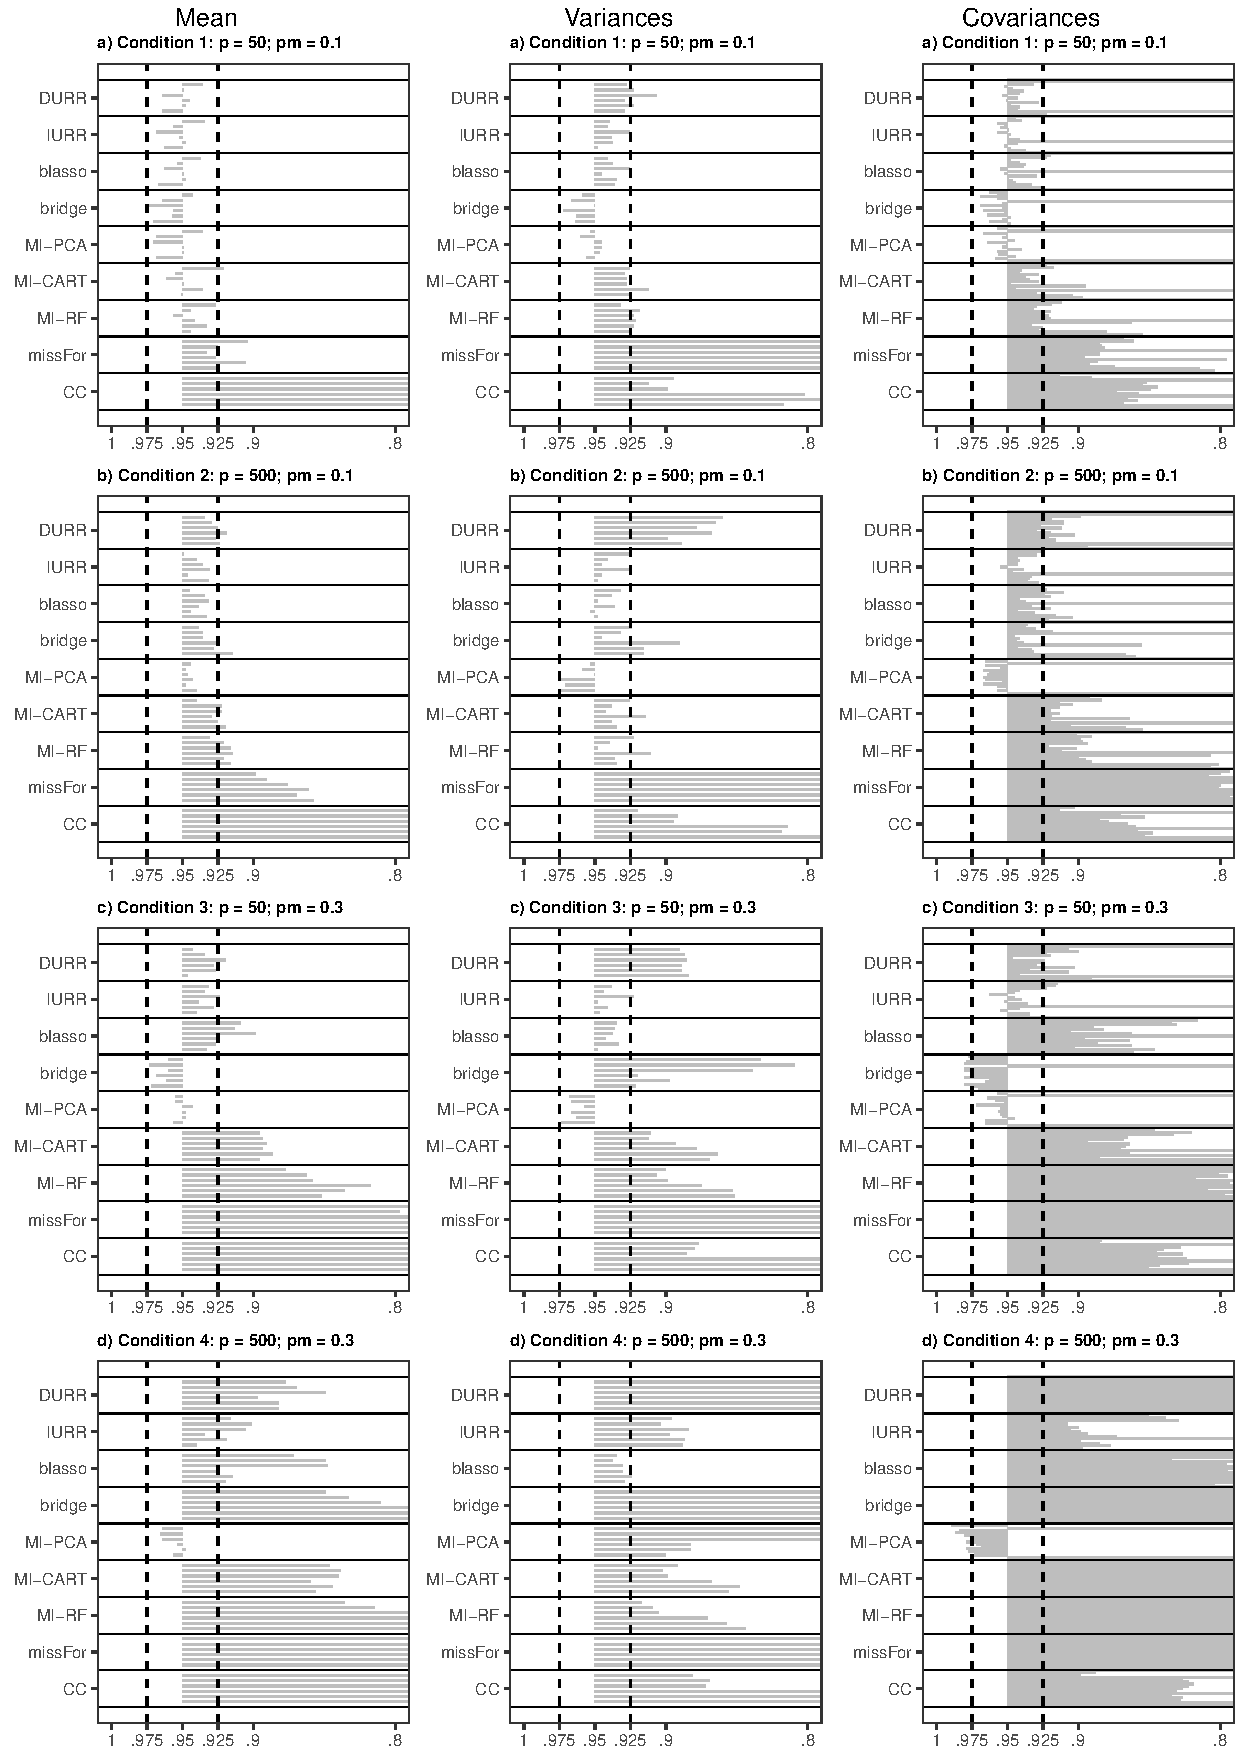
\includegraphics{../../output/graphs/exp1_CI.pdf}
\caption{Confidence Interval Coverage (CIC) for item means, variances, and covariances. 
	For every method, single horizontal lines, representing the CIC of a parameter estimate on 
	a single variable (or pair of variables), combine to form larger horizontal bars giving an 
	aggregate account of how each method performed across multiple variables with missing values.
}
\label{fig:exp1cir}
\end{figure}
	
\FloatBarrier % stops fig:exp1cir to leave its section
%\end{landscape}
%\end{rotatepage}

\subsubsection{Experiment 2}

	Figure \ref{fig:exp2bias} and \ref{fig:exp2cir} report the Percentage Relative Bias and Confidence Interval 
	Coverage, respectively, of the estimated means, variances, and covariances of the 10 observed items with
	missing values in the first four conditions of experiment 2, the ones with high factor loadings (strong 
	latent structure).
	In the figures, single horizontal lines, representing the PRB (or CIC) of a parameter estimate for a single variable, 
	combine to form larger horizontal bars giving an aggregate account of how each method performed across
	multiple variables with missing values.
	Figure \ref{fig:exp2bias58} and \ref{fig:exp2cir58} in appendix reports the same values for the low 
	factor loading conditions.

	\paragraph{Means}
	All methods provided unbiased estimates of the item means with PRBs that were almost 0 for all items.
	As the proportion of missing cases increased, in conditions 3 and 4, there was a slight increase in 
	PRB values for all methods except IURR, bridge, and MI-PCA. 
	However, only Complete Case analysis led to unacceptable bias in these scenarios.
	DURR, IURR and MI-PCA also showed little to no deviations from nominal coverage in all conditions, 
	while Blasso, MI-CART, MI-RF, and Bridge showed important sings of under-coverage when the proportion of 
	missing cases was high (conditions 3 and 4). 
	missForest also led to extreme under coverage of the true values.
	
	\paragraph{Variances}
	All MI methods, except Bridge, showed acceptable bias levels for item variances estimates in all conditions, 
	but the least biased estimates were obtained by MI-OP, IURR and MI-PCA.
	Confidence Intervals Coverage decreased as the proportion of missing cases increased (from condition 1 and 2 
	to conditions 3 and 4, respectively).
	For high $pm$, only IURR and MI-PCA maintained CICs mostly within the range .94-.96, with the former showing slight signs of 
	under-coverage and the latter tending toward over-coverage, while blasso and the MI tree-based methods showed sings of 
	mild and extreme under-coverage (CIC < 90\%), respectively.

	The large positive bias (and low CIC) for the item variances that afflicted MI-PCA in the multivariate-normal set up 
	(figures \ref{fig:exp1bias} and \ref{fig:exp1cir}) is not present in figures \ref{fig:exp2bias} and \ref{fig:exp2cir}.
	However, that pattern reappeared when the latent structure was weak, as can be seen in figure \ref{fig:exp2bias58} 
	and \ref{fig:exp2cir58} in the appendix (conditions 5 to 8, factor loadings between .5 and .8).

	Single data approaches, missForest and CC, showed again extreme (negative) bias and CI under-coverage in 
	almost all conditions.

	\paragraph{Covariances}

	IURR and DURR showed acceptable biases (PRBs below 10\% in absolute value) in conditions 1 to 4, but the 
	large negative covariance bias and extreme low coverage shown in the first experiment (see
	figures \ref{fig:exp1bias} and \ref{fig:exp1cir}) reappeared when the latent structure was weak, as can be seen in 
	figure \ref{fig:exp2bias58} and \ref{fig:exp2cir58} in the appendix (conditions 5 to 8, factor loadings 
	between .5 and .6).

	The other methods performed exactly as in experiment 1: the MI-PCA approach resulted in the lowest 
	bias and deviation from nominal coverage for the covariances of the observed items; 
	all other methods led to large negative biases and mild-to-extreme under-coverage for all the covariances, 
	in all conditions.

%\begin{rotatepage}	
\begin{figure}
	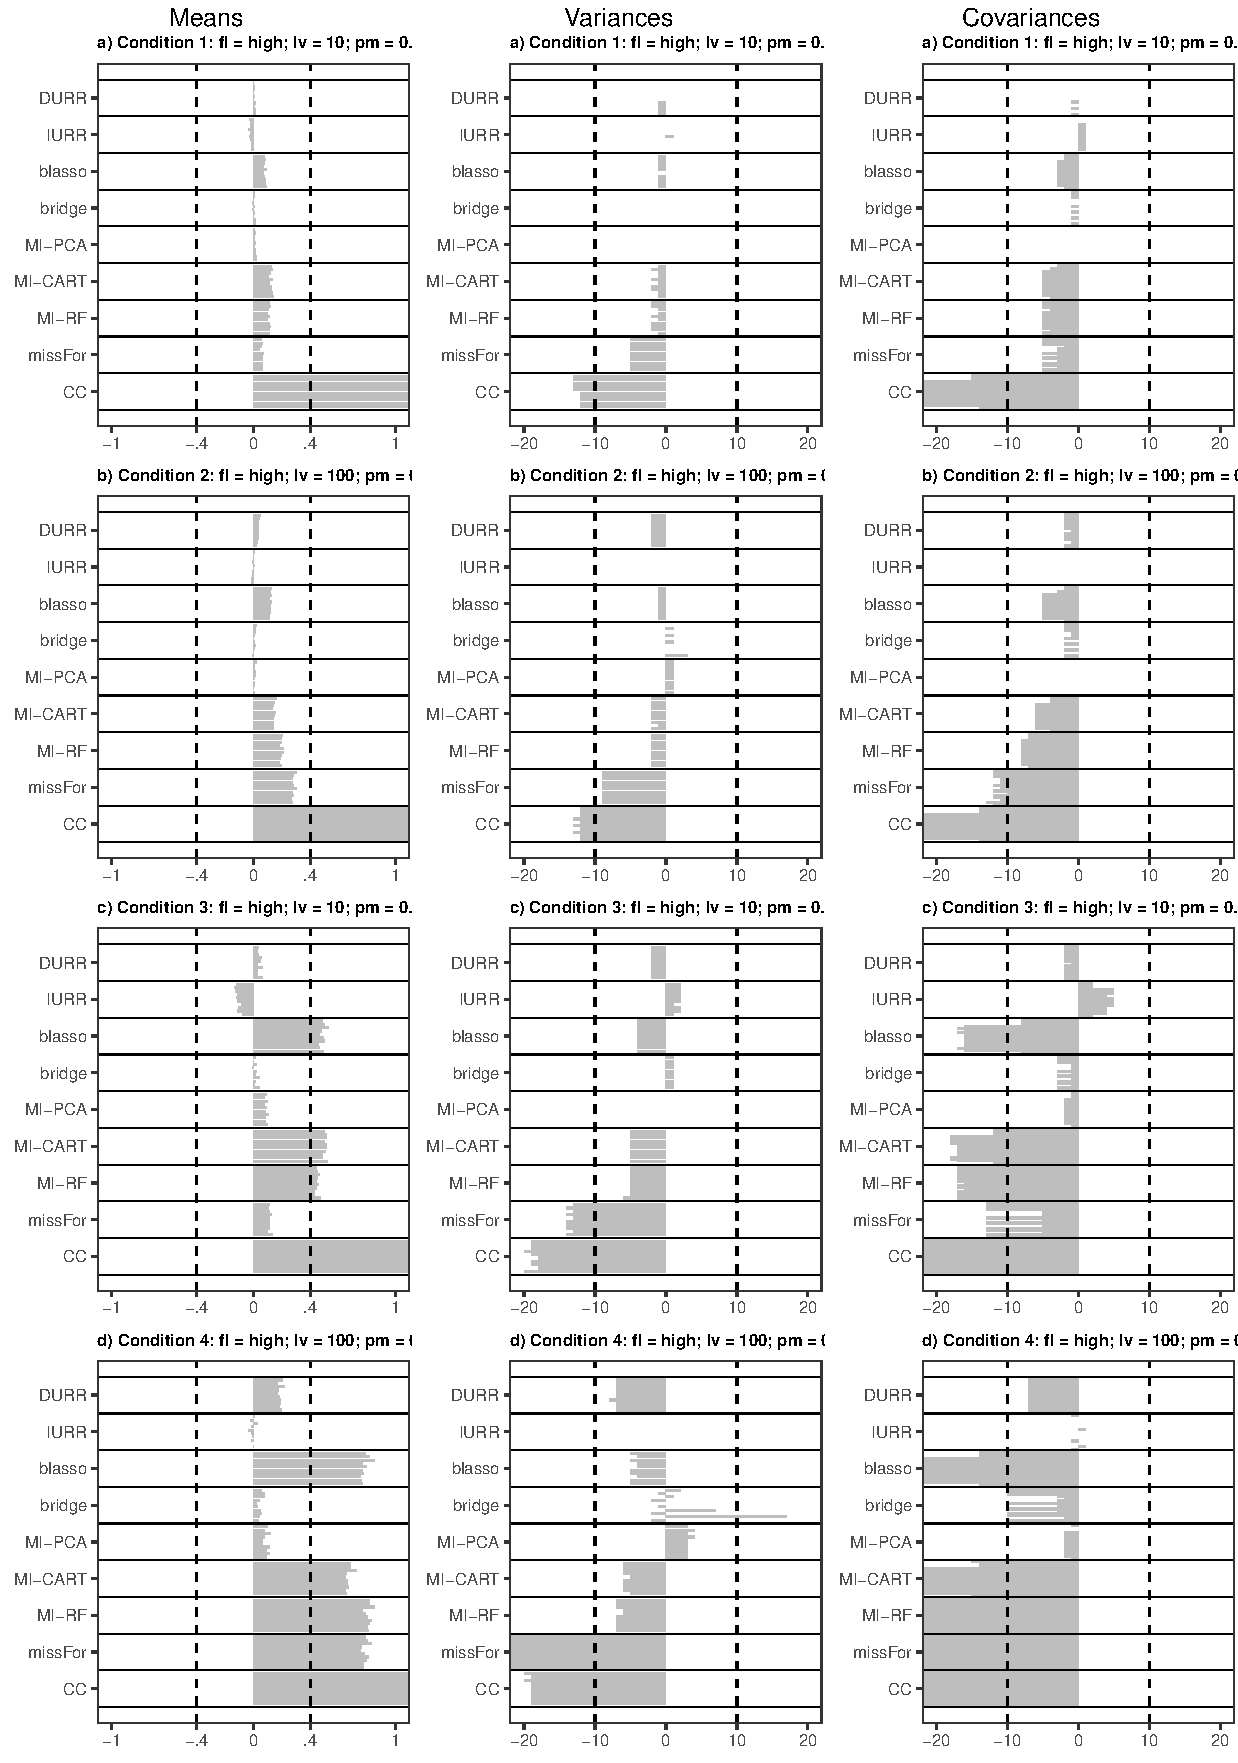
\includegraphics{../../output/graphs/exp2_semR_bias_14.pdf}
\caption{PRBs for the means, variances and covariances (PRB) for condition 1 to 4.
	For every method, single horizontal lines, representing the PRB of a parameter estimate on 
	a single variable (or pair of variables), combine to form larger horizontal bars giving an 
	aggregate account of how each method performed across multiple variables with missing values.
}
\label{fig:exp2bias}
\end{figure}

\begin{figure}
	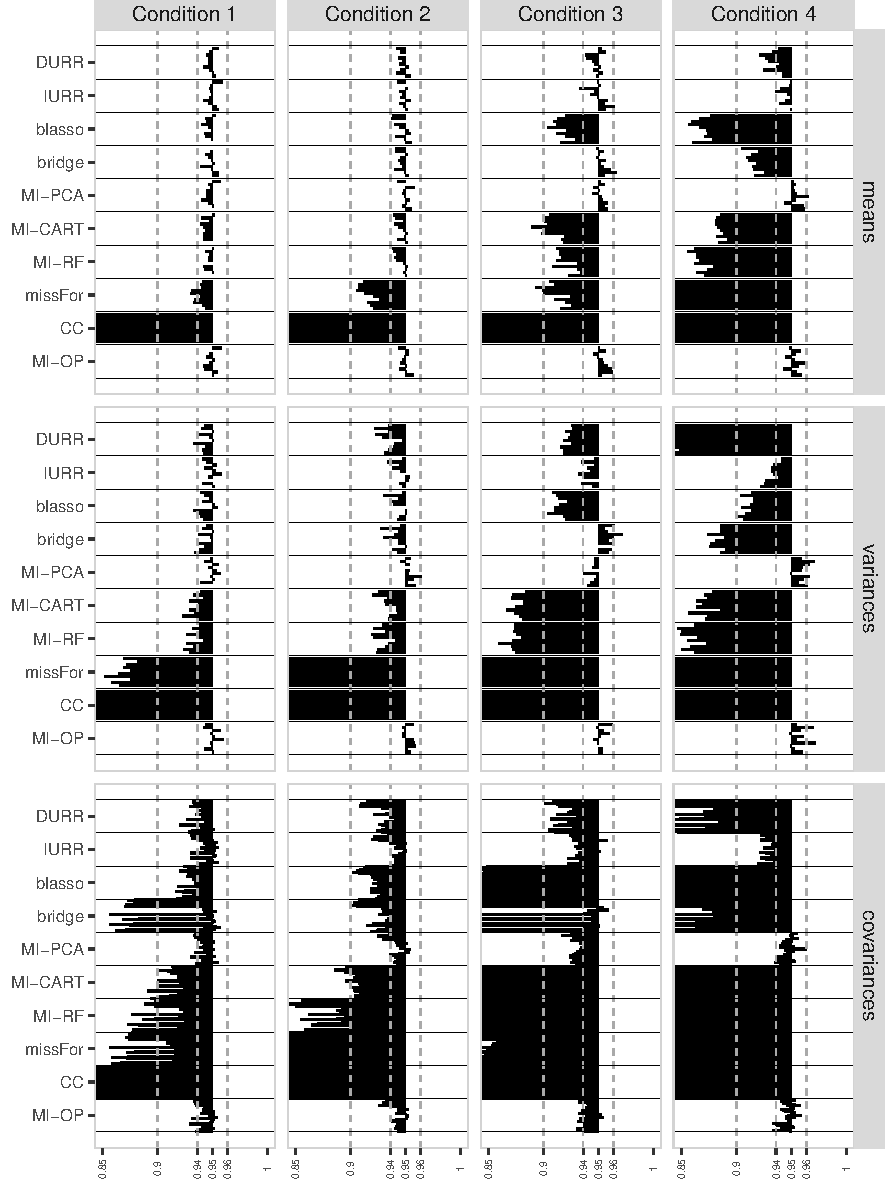
\includegraphics{../../output/graphs/exp2_semR_ci_14.pdf}
\caption{CIC for the means, variances, and covariances for condition 1 to 4.
	For every method, single horizontal lines, representing the CIC of a parameter estimate on 
	a single variable (or pair of variables), combine to form larger horizontal bars giving an 
	aggregate account of how each method performed across multiple variables with missing values.
}
\label{fig:exp2cir}
\end{figure}

\FloatBarrier % stops fig:exp2cir to leave its section
%\end{rotatepage}

	\paragraph{Factor Loadings}
	Figures \ref{fig:exp2fl14} shows the PRB values for all the factor loadings estimated by
	the Confirmatory Factor Analysis described above. 
	Most MI-Methods provided acceptably low bias for these estimates in all conditions except the one with 
	both large proportion of missing values and high dimensional input data matrix (condition 4 and 8).

	MI-OP, IURR, and MI-PCA outperformed all other methods giving virtually unbiased estimates
	of the factor loadings in all conditions.
	In particular, MI-PCA outperformed IURR when factor loadings were low (panel b, conditions 5 to 8), 
	maintaining inconsequential biases even when data was high-dimensional and the proportion of missing 
	values was high.

\begin{figure}[h]
	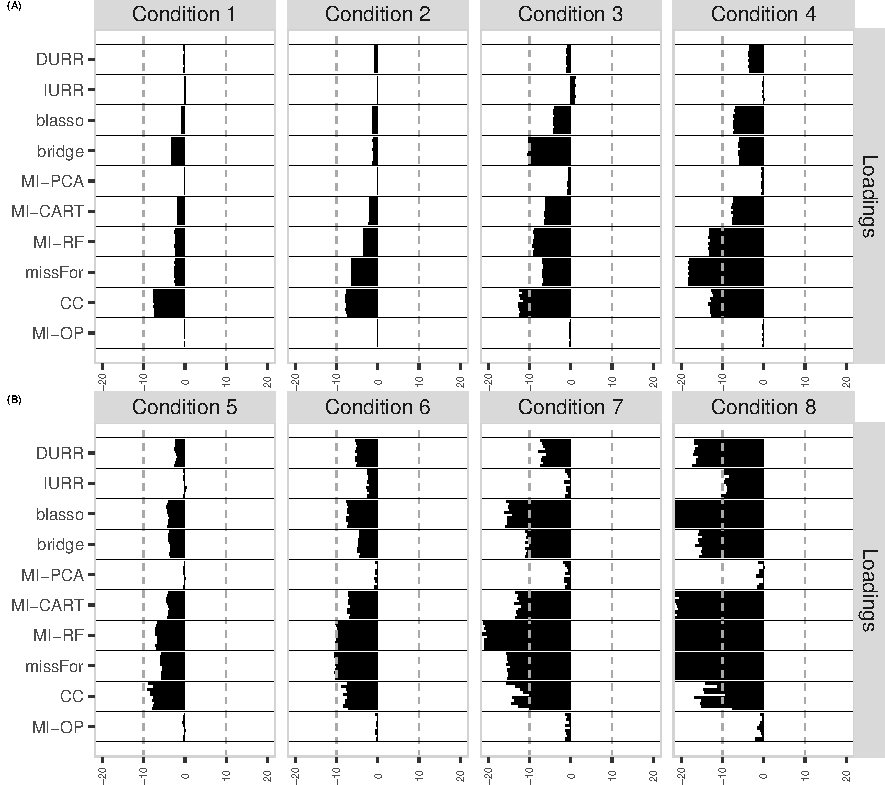
\includegraphics{../../output/graphs/exp2_CFA_lambda_BPR.pdf}
	\caption{
		Percent Relative Bias (PRB) for the factor loadings in conditions 1 to 4 (panel A) 
		and conditions 5 to 8 (panel B).
		Within each panel, for every method, single horizontal lines report the PRB of the 
		factor loading estimation for each item with missing values.
		}
\label{fig:exp2fl14}
\end{figure}

\FloatBarrier % stops fig:exp2fl to leave its section

